\section{Web Interface}
\label{sec:web_interface}

The web interface is a simple Django app, where researchers and scientists can register, upload and download images for the Captcha service to use.

\subsection{Upload}

The upload functionality allows for data to be uploaded for labeling or to feed tasks with already label data. The upload of pre-labeled data is necessary to guarantee the functionality of Captchas, thus the validation of a Captcha challenge.
First of all, the user chooses for which Captcha type he wants to upload his data and whether the data is already labeled or not.
For image Captchas, the User has to choose between an already existing task or he can add a task himself. The task declares which images are to be selected when solving the specific Captcha challenge.

For unsolved Captchas, the user simply has to upload a .zip-file with a folder containing his images. The .zip-file and the included folder need to have the same name.
For solved Captchas, the .zip-file must also contain a .txt-file (CSV). The .txt-file needs to containing each image name, followed with \verb|True| or \verb|False| for image Captchas, or their solution word for text Captchas, separated by a comma. If one of the images submitted is not included in the .txt-file it will be ignored. If the .txt-file contains an entry without a corresponding image in the image folder the upload will fail. 
\begin{figure}[H]
\centering
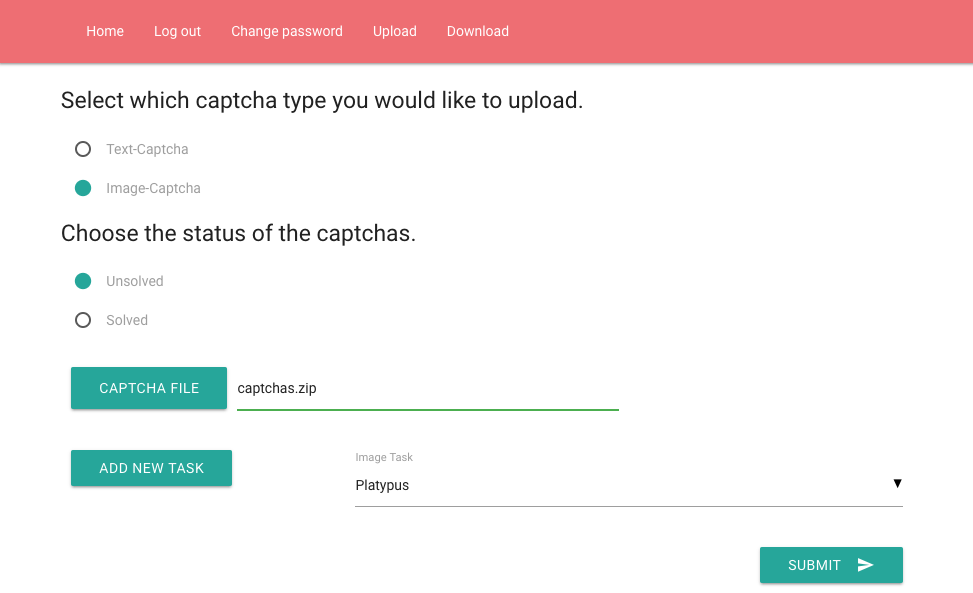
\includegraphics[width=1\linewidth]{content/figures/upload.png}
\caption{Upload page from web interface}
\label{fig:upload}
\end{figure}

\subsection{Download}

The download functionality allows for data to be downloaded by choosing the Captcha type. The researcher can specify his task for image Captchas, whereas that is not possible for text Captchas. By pressing the download button, all Captchas matching the chosen type and/or task are downloaded into a .zip-file, together with a .txt-file. For text Captchas, the .txt-file contains all images names followed with their labeled word. For image Captchas, the .txt-file contains all images names followed with \verb|True| or \verb|False|, whether they match their specific task.
\begin{figure}[H]
\centering
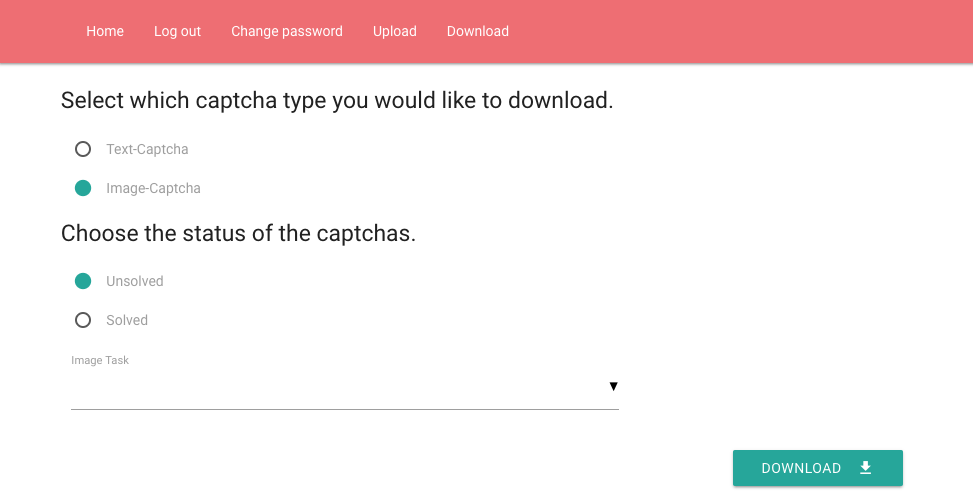
\includegraphics[width=1\linewidth]{content/figures/download.png}
\caption{Download page from web interface}
\label{fig:download}
\end{figure}

\subsection{User authentication and registration}

The user authentication and registration is built using the Django authentication system \footnote{https://docs.djangoproject.com/en/1.10/topics/auth/default/}. Users can register, whereby an Email-address is needed in order to minimize Spam. The authentication Email is sent from an Email-address, which is configured in settings.py.
The user receives an activation link, which is active for 7 days. After clicking the activation link, the user is able to login into the web interface.
\begin{figure}[H]
\centering
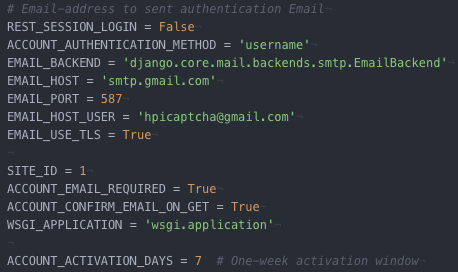
\includegraphics[width=0.8\linewidth]{content/figures/email_settings.png}
\caption{Email settings in settings.py}
\label{fig:email_settings}
\end{figure}

In order for the activation link to work, the site has to be configured within the Django administration. The site has to match the server address, where the Captcha service runs.
\begin{figure}[H]
\centering
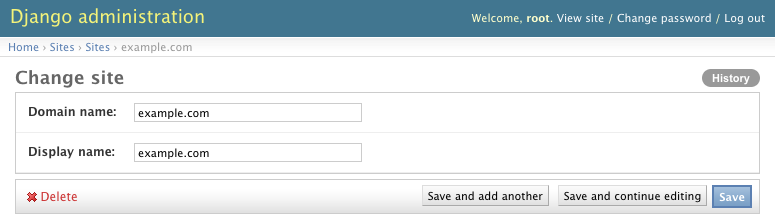
\includegraphics[width=1\linewidth]{content/figures/site_administration.png}
\caption{Configure site to match server address in the Django administration}
\label{fig:site_administration}
\end{figure}

\clearpage
